\newcommand{\QpuDocTitle}{Classical and Quantum Theory for QPU}
\newcommand{\QpuDocSubtitle}{From Bits to Bloch Spheres}
\newcommand{\QpuHeaderTitle}{Theory Guide}
\newcommand{\QpuDocDescription}{%
A ground-up explanation of classical logic, complex amplitudes, quantum state,
measurement, entanglement, mixed states and noise, and the mathematics
represented by QPU gates.
}
\documentclass[10pt,letterpaper]{article}

% Stable output supports docs:check even when translation uses a temporary directory.
\ifdefined\pdftrailerid
  \pdftrailerid{}
\fi

\usepackage[T1]{fontenc}
\usepackage[utf8]{inputenc}
\usepackage{lmodern}
\usepackage[margin=0.72in]{geometry}
\usepackage{amsmath,amssymb,mathtools}
\usepackage{booktabs,longtable,tabularx,array}
\usepackage[dvipsnames,table]{xcolor}
\usepackage{listings}
\usepackage{tikz}
\usepackage{enumitem}
\usepackage{fancyhdr}
\usepackage{microtype}
\usepackage[hidelinks]{hyperref}
\usepackage{bookmark}
\usepackage{titlesec}

\usetikzlibrary{arrows.meta,calc,positioning}

\definecolor{QpuNavy}{HTML}{0F172A}
\definecolor{QpuBlue}{HTML}{2563EB}
\definecolor{QpuCyan}{HTML}{0891B2}
\definecolor{QpuGreen}{HTML}{047857}
\definecolor{QpuAmber}{HTML}{B45309}
\definecolor{QpuRed}{HTML}{B91C1C}
\definecolor{QpuPaper}{HTML}{F8FAFC}
\definecolor{QpuLine}{HTML}{CBD5E1}
\definecolor{CodeBg}{HTML}{F1F5F9}
\definecolor{CodeComment}{HTML}{64748B}

\providecommand{\QpuDocTitle}{QPU Documentation}
\providecommand{\QpuDocSubtitle}{System Guide}
\providecommand{\QpuDocDescription}{A guide to the QPU circuit system.}
\providecommand{\QpuHeaderTitle}{QPU Documentation}

\hypersetup{
  pdftitle={\QpuDocTitle: \QpuDocSubtitle},
  pdfauthor={Bailey Forbes},
  pdfsubject={QPU protocol syntax, quantum gates, mathematics, and truth tables},
  pdfkeywords={QPU, quantum circuit, protocol, system syntax, truth table}
}

\pagestyle{fancy}
\fancyhf{}
\lhead{\textcolor{QpuNavy}{QPU Circuit Compiler}}
\rhead{\textcolor{QpuNavy}{\QpuHeaderTitle}}
\cfoot{\thepage}
\renewcommand{\headrulewidth}{0.3pt}

\titleformat{\section}{\Large\bfseries\color{QpuNavy}}{\thesection}{0.55em}{}
\titleformat{\subsection}{\large\bfseries\color{QpuBlue}}{\thesubsection}{0.5em}{}
\titleformat{\subsubsection}{\normalsize\bfseries\color{QpuCyan}}{\thesubsubsection}{0.45em}{}
\setlist{nosep,leftmargin=1.5em}
\setlength{\parindent}{0pt}
\setlength{\parskip}{4pt}
\setlength{\tabcolsep}{4pt}
\renewcommand{\arraystretch}{1.15}

\lstdefinelanguage{QPU}{
  morekeywords={
    PARAMS,MAIN-PROCESS,INCREASECYCLE,COMPILEPROCESS,FREE,SET,JOIN,SPLIT,
    CALL,DECLARECHILD,RUNCHILD,REC,TREC,RECUR,EXIT,IF,ELSE,ENDIF,RETURNVALS,ACCEPTVALS,MASTERVAL,SAVE_STATE,
    LOAD_STATE,CREATETOKEN,DELETETOKEN,X,Y,Z,H,S,T,CNOT,CCNOT,CZ,CY,
    SWAP,PHASE,RX,RY,RZ,CPHASE,MEASURE,NOT,AND,NAND,OR,XOR
  },
  sensitive=false,
  morecomment=[l]{\#},
  morecomment=[s]{/*}{*/},
  morestring=[b]"
}
\lstset{
  language=QPU,
  basicstyle=\ttfamily\small,
  keywordstyle=\bfseries\color{QpuBlue},
  commentstyle=\itshape\color{CodeComment},
  backgroundcolor=\color{CodeBg},
  frame=single,
  rulecolor=\color{QpuLine},
  framerule=0.4pt,
  xleftmargin=0.4em,
  framexleftmargin=0.35em,
  columns=fullflexible,
  keepspaces=true,
  showstringspaces=false,
  breaklines=true,
  aboveskip=5pt,
  belowskip=5pt
}

\newcommand{\code}[1]{\texttt{\detokenize{#1}}}
\newcommand{\ket}[1]{\lvert #1\rangle}
\newcommand{\bra}[1]{\langle #1\rvert}
\newcommand{\status}[1]{\textsf{\small #1}}
\newcommand{\implemented}{\textcolor{QpuGreen}{\status{lowered/executed}}}
\newcommand{\acceptedonly}{\textcolor{QpuAmber}{\status{accepted, not executed}}}
\newcommand{\internal}{\textcolor{QpuCyan}{\status{compiler-internal}}}

\newcommand{\GateSegment}[1]{%
\begin{tikzpicture}[baseline=-0.55ex,scale=.78]
  \draw[thick] (0,0)--(3.6,0);
  \node[left] at (0,0) {$\ket{q}$};
  \node[draw=QpuBlue,fill=QpuBlue!8,minimum width=.62cm,minimum height=.55cm,font=\bfseries] at (1.8,0) {#1};
\end{tikzpicture}}

\newcommand{\ControlledSegment}[1]{%
\begin{tikzpicture}[baseline=-0.55ex,scale=.78]
  \draw[thick] (0,.55)--(3.6,.55);
  \draw[thick] (0,-.55)--(3.6,-.55);
  \node[left] at (0,.55) {$\ket{c}$};
  \node[left] at (0,-.55) {$\ket{t}$};
  \fill[QpuNavy] (1.8,.55) circle (.09);
  \draw[thick] (1.8,.55)--(1.8,-.55);
  \node[draw=QpuBlue,fill=QpuBlue!8,circle,inner sep=1.7pt,font=\scriptsize\bfseries] at (1.8,-.55) {#1};
\end{tikzpicture}}

\newcommand{\DoubleControlledSegment}{%
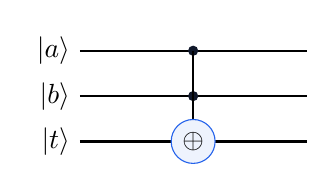
\begin{tikzpicture}[baseline=-0.55ex,scale=.72]
  \foreach \y/\n in {.8/a,0/b,-.8/t} {
    \draw[thick] (0,\y)--(4,\y);
    \node[left] at (0,\y) {$\ket{\n}$};
  }
  \fill[QpuNavy] (2,.8) circle (.09);
  \fill[QpuNavy] (2,0) circle (.09);
  \draw[thick] (2,.8)--(2,-.8);
  \node[draw=QpuBlue,fill=QpuBlue!8,circle,inner sep=2pt,font=\bfseries] at (2,-.8) {$\oplus$};
\end{tikzpicture}}

\newcommand{\SwapSegment}{%
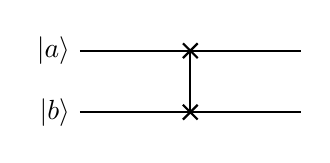
\begin{tikzpicture}[baseline=-0.55ex,scale=.78]
  \draw[thick] (0,.5)--(3.6,.5);
  \draw[thick] (0,-.5)--(3.6,-.5);
  \node[left] at (0,.5) {$\ket{a}$};
  \node[left] at (0,-.5) {$\ket{b}$};
  \draw[thick] (1.68,.38)--(1.92,.62) (1.68,.62)--(1.92,.38);
  \draw[thick] (1.68,-.38)--(1.92,-.62) (1.68,-.62)--(1.92,-.38);
  \draw[thick] (1.8,.5)--(1.8,-.5);
\end{tikzpicture}}

\newcommand{\QpuMeter}[2]{%
  \begin{scope}[shift={(#1,#2)}]
    \draw[QpuBlue,thick] (-0.28,-0.22) rectangle (0.28,0.28);
    \draw[QpuBlue,thick] (-0.18,-0.02) arc (180:0:0.18);
    \draw[QpuBlue,thick] (0,-0.02) -- (0.14,0.16);
    \fill[QpuBlue] (0,-0.02) circle (0.035);
  \end{scope}}
\newcommand{\MeasureSegment}{%
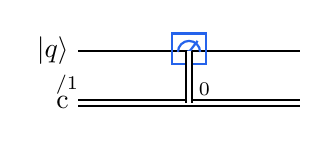
\begin{tikzpicture}[baseline=-0.55ex,scale=.78]
  \draw[thick] (0,0)--(3.6,0);
  \node[left] at (0,0) {$\ket{q}$};
  \QpuMeter{1.8}{0}
  \draw[double distance=1.4pt,thick] (0,-.85)--(3.6,-.85);
  \node[left] at (0,-.85) {c};
  \node[left,font=\scriptsize] at (0.15,-.55) {/1};
  \draw[double distance=1.4pt,thick] (1.8,0)--(1.8,-.85);
  \node[right,font=\scriptsize] at (1.8,-.62) {0};
\end{tikzpicture}}

% The hypertarget gives each gate a stable PDF named destination (gate-CNOT,
% gate-H, ...) that the workbench links to with #nameddest=.
\newcommand{\GateHeading}[3]{%
\subsection{#1 (\code{#2})}\hypertarget{gate-#2}{}
\begin{center}#3\end{center}}

% Short framed callouts. The body is boxed, so it cannot contain lstlisting
% and should stay short enough to fit on one page.
\newsavebox{\QpuCalloutBox}
\newenvironment{QpuCallout}[2]{%
  \def\QpuCalloutColor{#1}%
  \setlength{\fboxrule}{0.6pt}%
  \par\smallskip\noindent
  \begin{lrbox}{\QpuCalloutBox}%
  \begin{minipage}{\dimexpr\linewidth-2\fboxsep-2\fboxrule\relax}%
  \setlength{\parskip}{3pt}%
  {\bfseries\color{#1}#2}\par
}{%
  \end{minipage}%
  \end{lrbox}%
  \fcolorbox{\QpuCalloutColor}{\QpuCalloutColor!6}{\usebox{\QpuCalloutBox}}%
  \par\smallskip
}
\newenvironment{beginnerbox}[1][Beginner note]{\begin{QpuCallout}{QpuGreen}{#1}}{\end{QpuCallout}}
\newenvironment{trybox}[1][Try it in the Circuit builder]{\begin{QpuCallout}{QpuBlue}{#1}}{\end{QpuCallout}}
\newenvironment{cautionbox}[1][Watch out]{\begin{QpuCallout}{QpuAmber}{#1}}{\end{QpuCallout}}

% Workbench selectors on the left, the circuit diagram they produce on the
% right. #1 is the gate name shown in the Gate selector and on the target.
\newcommand{\WorkbenchControlMap}[1]{%
\begin{tikzpicture}[font=\small,>={Latex[length=2mm]}]
  \tikzset{ui/.style={draw=##1,rounded corners=2pt,anchor=west,minimum width=3.9cm,minimum height=.55cm,inner sep=3pt}}
  \node[ui=QpuLine,fill=CodeBg] at (0,1.75) {\textsf{Gate:} \textbf{#1}};
  \node[ui=QpuBlue,fill=QpuBlue!8] (a) at (0,.95) {\textsf{Control A:} \textbf{q0}};
  \node[ui=QpuBlue,fill=QpuBlue!8] (b) at (0,.15) {\textsf{Control B:} \textbf{q1}};
  \node[ui=QpuRed,fill=QpuRed!6] (t) at (0,-.65) {\textsf{Target particle:} \textbf{q2}};
  \node[font=\scriptsize\bfseries,color=QpuNavy,anchor=west] at (0,2.45) {Interactive workbench};
  \node[font=\scriptsize\bfseries,color=QpuNavy] at (7.4,2.45) {Circuit canvas};
  \foreach \y/\q in {.95/q0,.15/q1,-.65/q2} {
    \draw[thick] (5.6,\y)--(9.2,\y);
    \node[left,font=\scriptsize] at (5.6,\y) {\q};
  }
  \draw[->,dashed,QpuBlue] (a.east)--(5.05,.95);
  \draw[->,dashed,QpuBlue] (b.east)--(5.05,.15);
  \draw[->,dashed,QpuRed] (t.east)--(5.05,-.65);
  \fill[QpuNavy] (7.4,.95) circle (.09);
  \fill[QpuNavy] (7.4,.15) circle (.09);
  \draw[thick] (7.4,.95)--(7.4,-.65);
  \node[draw=QpuRed,fill=QpuRed!6,circle,inner sep=1.5pt,font=\bfseries] at (7.4,-.65) {$\oplus$};
  \node[anchor=west,font=\scriptsize] at (9.3,.95) {$A$: read, left unchanged};
  \node[anchor=west,font=\scriptsize] at (9.3,.15) {$B$: read, left unchanged};
  \node[anchor=west,font=\scriptsize] at (9.3,-.65) {$t' = t\oplus(A\land B)$: written};
\end{tikzpicture}}

\newcommand{\QpuTitlePage}{%
\begin{titlepage}
\pagecolor{QpuPaper}
\centering
\vspace*{1.15in}
{\Huge\bfseries\color{QpuNavy} \QpuDocTitle\par}
\vspace{0.2in}
{\LARGE\color{QpuBlue} \QpuDocSubtitle\par}
\vspace{0.55in}
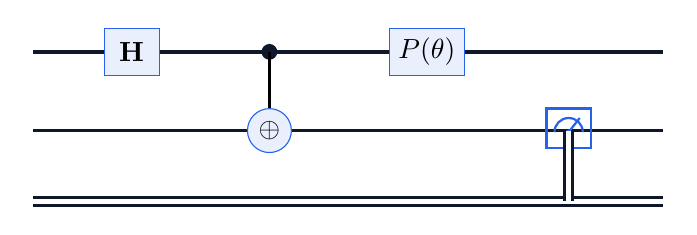
\begin{tikzpicture}
  \draw[very thick,QpuNavy] (0,1)--(8,1);
  \draw[very thick,QpuNavy] (0,0)--(8,0);
  \draw[double distance=1.6pt,very thick,QpuNavy] (0,-.9)--(8,-.9);
  \node[draw=QpuBlue,fill=QpuBlue!10,minimum width=.7cm,minimum height=.6cm,font=\bfseries] at (1.25,1) {H};
  \fill[QpuNavy] (3,1) circle (.1);
  \draw[very thick] (3,1)--(3,0);
  \node[draw=QpuBlue,fill=QpuBlue!10,circle,inner sep=2pt] at (3,0) {$\oplus$};
  \node[draw=QpuBlue,fill=QpuBlue!10,minimum width=.8cm,minimum height=.6cm,font=\bfseries] at (5,1) {$P(\theta)$};
  \QpuMeter{6.8}{0}
  \draw[double distance=1.6pt,very thick,QpuNavy] (6.8,0)--(6.8,-.9);
\end{tikzpicture}
\vfill
{\large Bailey Forbes\par}
{\large September 13, 2026\par}
\vspace{0.35in}
\begin{minipage}{0.82\textwidth}
\small\color{QpuNavy}
\QpuDocDescription
\end{minipage}
\vfill
\end{titlepage}
\nopagecolor
}

% Widen the TOC number column so two-digit subsections (13.10) keep a gap before the title.
\makeatletter
\renewcommand*\l@subsection{\@dottedtocline{2}{1.5em}{2.8em}}
\renewcommand*\l@subsubsection{\@dottedtocline{3}{4.3em}{3.6em}}
\makeatother

\newcommand{\QpuContents}{%
\pagenumbering{roman}
\tableofcontents
\clearpage
\pagenumbering{arabic}
}


\begin{document}
\QpuTitlePage
\QpuContents

\section{Classical computation foundations}

Quantum circuits build on ideas from classical digital logic. Understanding
bits, Boolean functions, truth tables, and reversible computation makes the
QPU gate model much easier to use.

\subsection{Classical bits and logical state}

A classical bit has one definite logical value:
\[
b\in\{0,1\}.
\]
Physical computers may represent that value with voltage, charge, magnetic
orientation, or another measurable quantity. Digital logic ignores most
physical detail and works with the abstraction 0 or 1.

A wire carries a bit from one operation to another. A \emph{gate} computes a
function of one or more incoming bits. For example, NOT has one input and one
output:
\[
\operatorname{NOT}(0)=1,\qquad \operatorname{NOT}(1)=0.
\]
In QPU source, a token names the logical wire. On computational-basis states,
\code{X -I Q -O Q} has the same measured input/output relationship as
classical NOT.

\subsection{Boolean algebra}

Boolean algebra describes functions whose values are 0 and 1. This guide uses:
\begin{center}
\begin{tabularx}{\textwidth}{>{\bfseries}l c l X}
\toprule
Operation & Symbol & Spoken form & Meaning\\
\midrule
NOT & $\neg A$ & not A & 1 when A is 0; 0 when A is 1.\\
AND & $A\land B$ & A and B & 1 only when both inputs are 1.\\
OR & $A\lor B$ & A or B & 1 when either or both inputs are 1.\\
XOR & $A\oplus B$ & A exclusive-or B & 1 when exactly one input is 1.\\
NAND & $\neg(A\land B)$ & not-and & The complement of AND.\\
\bottomrule
\end{tabularx}
\end{center}

For bits, XOR is addition modulo two:
\[
0\oplus0=0,\quad 0\oplus1=1,\quad
1\oplus0=1,\quad 1\oplus1=0.
\]
There is no carry in modulo-two addition. Ordinary binary addition handles the
carry separately, which is why a half-adder produces both Sum and Carry.

\subsection{Truth tables as complete finite specifications}

A truth table lists a function's output for every possible input pattern. With
$n$ binary inputs there are $2^n$ patterns. AND, OR, XOR, and NAND can be
compared in one table:
\begin{center}
\begin{tabular}{cc|cccc}
\toprule
$A$&$B$&$A\land B$&$A\lor B$&$A\oplus B$&$\neg(A\land B)$\\
\midrule
0&0&0&0&0&1\\
0&1&0&1&1&1\\
1&0&0&1&1&1\\
1&1&1&1&0&0\\
\bottomrule
\end{tabular}
\end{center}
For a deterministic combinational circuit, this table completely specifies
the classical input/output behavior. It does not reveal the circuit's internal
gate arrangement, propagation time, power consumption, or quantum phase.

\subsection{Combinational logic and stored state}

A \emph{combinational} output depends only on current inputs. Adders and the
Boolean gates above are combinational. A \emph{sequential} circuit also depends
on stored state from an earlier step, as in counters and latches.

QPU cycle suffixes can document successive stages, and INCREASECYCLE marks a
workspace boundary, but the compiled circuit is still one ordered gate
sequence. \code{SAVE_STATE} and \code{LOAD_STATE} copy and restore the simulator
state vector. They are not quantum gates. When modeling stateful behavior
inside the unitary circuit, expose previous state as PARAMS and return next
state through RETURNVALS.

\subsection{Why ordinary classical gates can lose information}

A function is reversible only if each output identifies exactly one input.
Classical NOT is reversible: seeing output 1 proves the input was 0. AND is not:
output 0 could have come from 00, 01, or 10.

\[
(A,B)\xrightarrow{\mathrm{AND}}A\land B
\]
maps four input patterns onto only two output values, discarding information.
Quantum evolution through closed-system gates must be unitary and therefore
reversible. A quantum/reversible AND preserves both inputs and mutates another
target:
\[
(A,B,t)\longmapsto(A,B,t\oplus(A\land B)).
\]
Knowing the output triple lets the transformation be run backward to recover
the input triple. This one-to-one property is one of four conditions a
quantum gate must satisfy to be reversible; \emph{Requirements for a
reversible gate}, in the Theory Guide's mathematical foundations chapter,
states all four together.

\begin{beginnerbox}[How to read $t' = t\oplus(A\land B)$]
\begin{itemize}
  \item $A$ and $B$ are \textbf{controls}. They are only read. After the gate
  they still hold exactly what they held before, which is why the input can
  always be recovered.
  \item $t$ is the \textbf{target}, the output workspace. It is the only wire
  that changes. The prime in $t'$ means ``$t$ after the gate''.
  \item $\oplus$ means ``flip if''. The target flips when $A\land B$ is 1 and
  stays put otherwise.
  \item Start the target at 0 and it ends holding $A\land B$, the ordinary AND
  answer. Start it at 1 and it ends holding NAND instead.
\end{itemize}
In the Circuit builder, $A$ is \textbf{Control A}, $B$ is
\textbf{Control B}, and $t$ is \textbf{Target particle}.
\end{beginnerbox}

\subsection{Controls, targets, and workspace}

These terms connect classical logic to QPU syntax:
\begin{description}
  \item[Control] A wire whose value decides whether a target operation occurs.
  In \code{CNOT -I A -O T}, A is the control.
  \item[Target] The wire changed by an operation. T is the target in that CNOT.
  \item[Workspace or ancilla] An extra wire introduced to hold an intermediate
  or output while preserving inputs. It is commonly initialized to $\ket0$.
  \item[Garbage] Intermediate information left in workspace after the desired
  answer has been computed. Reversible algorithms often \emph{uncompute}
  temporary gates to return garbage wires to zero.
  \item[Uncomputation] Applying inverse operations in reverse order to clean
  workspace without erasing information irreversibly.
\end{description}

The QPU language calls logical wire names tokens. \code{CREATETOKEN} reserves
workspace, SET prepares it, \code{-I} lists inputs/controls, and \code{-O}
names targets.

\subsection{Fan-out, copying, and the no-cloning boundary}

Classical logic freely copies a bit onto several wires. If the source is a
known basis bit and targets begin at zero, CNOT reproduces that basis value:
\[
\ket{x}\ket0\xrightarrow{\mathrm{CNOT}}\ket{x}\ket{x},
\qquad x\in\{0,1\}.
\]
For a superposition $\alpha\ket0+\beta\ket1$, the same circuit produces
\[
\alpha\ket{00}+\beta\ket{11},
\]
not
\[
(\alpha\ket0+\beta\ket1)\otimes
(\alpha\ket0+\beta\ket1).
\]
The first state is generally entangled; the second would be two independent
copies and contains cross terms. The no-cloning theorem forbids a universal
gate that copies every unknown quantum state. QPU aliases similarly give two
names to one wire; they do not create a physical copy.

\subsection{Deterministic, probabilistic, and quantum models}

\begin{tabularx}{\textwidth}{>{\bfseries}p{0.19\textwidth}XXX}
\toprule
Model & State description & Transformation & Observation\\
\midrule
Deterministic classical & One definite bit string & Boolean function &
The definite output bits\\
Probabilistic classical & Probabilities over bit strings & Stochastic update &
A sampled string\\
Pure-state quantum & Complex amplitudes over basis strings & Unitary matrix &
A sampled string after magnitude-squared probabilities and collapse\\
\bottomrule
\end{tabularx}

Negative and imaginary amplitudes are not negative or imaginary probabilities.
They carry phase. Two computational paths can add constructively or cancel
destructively before probabilities are calculated. This interference has no
counterpart in an ordinary classical random-choice table.

\subsection{Classical and QPU operation map}

\begin{center}
\begin{tabularx}{\textwidth}{>{\bfseries}l l X}
\toprule
Classical idea & QPU operation & Important difference\\
\midrule
NOT & X or NOT & Acts linearly on superpositions; X is unitary.\\
XOR into target & CNOT & Preserves the control and can entangle.\\
AND into target & CCNOT or AND & Preserves controls; target is XOR-mutated.\\
Swap variables & SWAP & Exchanges complete quantum wire states.\\
Random bit & H then MEASURE & H first creates coherent amplitudes, not an
ordinary hidden random choice.\\
Read a bit & MEASURE & Sampling collapses a superposition and can disturb
entanglement.\\
Initialize zero & SET token 0p & Compiles to state preparation/reset behavior.\\
Function output & RETURNVALS & Declares an interface; does not itself copy or
measure a wire.\\
\bottomrule
\end{tabularx}
\end{center}


\section{Mathematical foundations}

This chapter assumes no prior quantum mechanics. The essential ideas are
numbers, vectors, probability, and transformations. Quantum notation can look
unfamiliar, but each symbol has a concrete computational meaning.

\subsection{Real numbers and complex numbers}

The real numbers include familiar values such as $-2$, $0$, $1/3$, and
$\sqrt2$. A real number can be placed on a one-dimensional number line.
Quantum amplitudes require a second numerical direction, represented by the
\emph{imaginary unit}
\[
i=\sqrt{-1},\qquad i^2=-1.
\]
There is no real number whose square is $-1$, so $i$ extends the number system.
A complex number has the form
\[
z=a+bi,
\]
where $a$ is the real part and $b$ is the imaginary part. Examples are
$3+2i$, $-i$, and $1$ (which is $1+0i$).

Complex arithmetic follows ordinary algebra together with $i^2=-1$:
\[
(a+bi)+(c+di)=(a+c)+(b+d)i,
\]
\[
(a+bi)(c+di)=(ac-bd)+(ad+bc)i.
\]
For example,
\[
(1+i)^2=1+2i+i^2=2i.
\]

\subsection{The complex plane, magnitude, and conjugate}

A complex number is a point or arrow in a plane: horizontal coordinate $a$,
vertical coordinate $b$. Its magnitude is the arrow length,
\[
|z|=\sqrt{a^2+b^2}.
\]
The complex conjugate reflects the arrow across the real axis:
\[
z^*=a-bi.
\]
Multiplying by the conjugate gives a nonnegative real number:
\[
z^*z=(a-bi)(a+bi)=a^2+b^2=|z|^2.
\]
Quantum measurement probabilities use $|z|^2$, not $z$ itself. This guarantees
real, nonnegative probabilities even though amplitudes may be complex.

\subsection{Angles, radians, sine, and cosine}

An arrow in the complex plane may be described by its length $r$ and angle
$\theta$:
\[
a=r\cos\theta,\qquad b=r\sin\theta.
\]
Quantum formulas normally measure angles in radians. One full turn is $2\pi$
radians, a half turn is $\pi$, and a quarter turn is $\pi/2$. Conversion is
\[
\theta_{\rm radians}=\theta_{\rm degrees}\frac{\pi}{180}.
\]
This is why \code{PHASE=90d} and \code{PHASE=pi/2} describe the same angle.

\subsection{Euler's formula and Euler's identity}

Euler's formula connects complex numbers to rotations:
\[
e^{i\theta}=\cos\theta+i\sin\theta.
\]
The value $e^{i\theta}$ always has magnitude one. As $\theta$ changes, it moves
around the unit circle in the complex plane. Important cases are
\[
e^{i0}=1,\quad e^{i\pi/2}=i,\quad e^{i\pi}=-1,\quad
e^{i2\pi}=1.
\]
Setting $\theta=\pi$ gives Euler's identity,
\[
e^{i\pi}+1=0.
\]
In a phase gate, multiplying an amplitude by $e^{i\theta}$ rotates that
amplitude without changing its magnitude. Its immediate measurement
probability is unchanged, but its relationship to other amplitudes changes.
Later gates can convert that relative phase into different probabilities.

\subsection{Vectors and basis vectors}

A column vector is an ordered list of numbers. The two basis vectors used for
one qubit are
\[
\ket0=\begin{bmatrix}1\\0\end{bmatrix},\qquad
\ket1=\begin{bmatrix}0\\1\end{bmatrix}.
\]
The vertical bars and angle bracket form Dirac's \emph{ket} notation.
\code{0p} prepares $\ket0$ and \code{1p} prepares $\ket1$.
Any one-qubit pure state is a complex linear combination:
\[
\ket{\psi}=\alpha\ket0+\beta\ket1
=\begin{bmatrix}\alpha\\\beta\end{bmatrix}.
\]
The complex numbers $\alpha$ and $\beta$ are \emph{probability amplitudes}.
They are not probabilities themselves.

\subsection{Normalization and the Born rule}

A valid state is normalized:
\[
|\alpha|^2+|\beta|^2=1.
\]
The Born rule turns amplitudes into measurement probabilities:
\[
P(0)=|\alpha|^2,\qquad P(1)=|\beta|^2.
\]
For the plus state,
\[
\ket+=\frac{\ket0+\ket1}{\sqrt2},
\]
both amplitudes are $1/\sqrt2$. Squaring their magnitudes gives
$P(0)=P(1)=1/2$. The factor $1/\sqrt2$ is therefore required; writing
$\ket0+\ket1$ without normalization would produce total probability two.

\subsection{Matrices as gates}

A matrix is a rectangular array of numbers. A one-qubit gate is represented by
a $2\times2$ complex matrix. Matrix-vector multiplication computes the new
amplitudes:
\[
\begin{bmatrix}a&b\\c&d\end{bmatrix}
\begin{bmatrix}\alpha\\\beta\end{bmatrix}
=
\begin{bmatrix}a\alpha+b\beta\\c\alpha+d\beta\end{bmatrix}.
\]
For example, the X gate exchanges the two amplitudes:
\[
\begin{bmatrix}0&1\\1&0\end{bmatrix}
\begin{bmatrix}\alpha\\\beta\end{bmatrix}
=\begin{bmatrix}\beta\\\alpha\end{bmatrix}.
\]
Applying gates in source order means multiplying by matrices in the same
temporal order: if U acts first and V second, then
\[
\ket{\psi_{\rm final}}=V(U\ket{\psi_{\rm initial}})=VU\ket{\psi_{\rm initial}}.
\]

\subsection{Requirements for a reversible gate}
\hypertarget{gate-reversibility-requirements}{}

A quantum gate is, by default, reversible: closed-system evolution is unitary,
and unitarity already implies everything ``reversible'' requires. The four
conditions below are one fact, stated four ways --- as a matrix equation, as a
statement about information, as a wire count, and as a scope limit --- so that
each can be checked on its own.

\begin{enumerate}
  \item \textbf{Unitarity.} The gate's matrix $U$ must satisfy
  \[
  U^\dagger U=UU^\dagger=I,
  \]
  where $U^\dagger$ transposes $U$ and complex-conjugates every entry
  (\emph{The complex plane, magnitude, and conjugate}), and $I$ is the
  identity matrix. Unitarity guarantees an inverse, $U^{-1}=U^\dagger$: the
  gate's action can always be undone by running $U^\dagger$. It is also
  exactly the condition that keeps a state normalized
  ($|\alpha|^2+|\beta|^2=1$, \emph{Normalization and the Born rule}) after the
  gate runs, so the total probability of all outcomes stays $100\%$.

  \item \textbf{Bijective mapping.} The gate must be a one-to-one map from
  input states to output states: given only the output and the gate, the
  input can always be reconstructed. Classical NOT has this property (an
  output of 1 proves the input was 0); classical AND and OR do not (an output
  of 0 does not say which inputs produced it), which is why they are not
  themselves reversible. A gate satisfying $U^\dagger U=I$ automatically has
  this property, because $U^\dagger$ is precisely the map that reconstructs
  the input from the output. Unitarity and bijectivity are the same fact
  viewed two ways; a reversible gate never erases information.

  \item \textbf{Equal inputs and outputs.} $U$ is a square matrix, so a
  reversible gate has exactly as many output wires as input wires: no wire
  can be discarded mid-computation without breaking the bijection above. This
  is why QPU's \code{AND} is not the two-input classical gate but a
  three-wire embedding,
  \[
  \ket{a,b,t}\mapsto\ket{a,b,t\oplus(a\land b)},
  \]
  the doubly-controlled CCNOT/Toffoli gate
  (\hyperlink{ccnot-and-embedding}{Doubly controlled NOT / Toffoli}). With
  $t$ starting at $\ket0$, $t'=a\land b$: the classical AND is recovered on
  $t'$ without erasing $a$ or $b$, at the cost of one extra wire the
  two-input classical gate did not need.

  \item \textbf{Isolation from measurement.} The three conditions above hold
  only for a closed system, with no interaction with the environment and, in
  particular, no MEASURE (\hyperlink{measure-collapse}{Measurement gate}).
  Measurement is not linear and has no inverse matrix: it collapses a
  superposition to one classical outcome and permanently discards the
  amplitudes that were not observed. RESET shares this --- preparing a wire
  at $\ket0$ regardless of its prior state is not invertible either
  (\hyperlink{reset-semantics}{Reversible gates versus RESET}). MEASURE and
  RESET are legitimate operations, just not reversible ones, and they are the
  only two exceptions to an otherwise-unitary gate list.
\end{enumerate}


\section{Qubits, phase, and the Bloch sphere}

\subsection{A qubit is not just an unknown bit}

A classical bit is exactly 0 or 1. A qubit may be in any normalized
superposition $\alpha\ket0+\beta\ket1$. This does not mean that the qubit
secretly chose a classical value before measurement. Relative amplitudes can
interfere, producing effects no ordinary random bit can reproduce.

\subsection{Global phase and relative phase}

Multiplying an entire state by a unit complex number does not change physical
predictions:
\[
\ket{\psi}\quad\text{and}\quad e^{i\gamma}\ket{\psi}
\]
have the same measurement probabilities and are considered equivalent up to a
\emph{global phase}. Relative phase is different. The states
\[
\ket+=\frac{\ket0+\ket1}{\sqrt2},\qquad
\ket-=\frac{\ket0-\ket1}{\sqrt2}
\]
give equal 0/1 probabilities if measured immediately, yet H sends
$\ket+\mapsto\ket0$ and $\ket-\mapsto\ket1$. Their relative sign is observable
through interference.

\subsection{Bloch-sphere coordinates}

After removing an unobservable global phase, every pure one-qubit state can be
written with two real angles:
\[
\ket{\psi}=
\cos\left(\frac{\theta}{2}\right)\ket0+
e^{i\phi}\sin\left(\frac{\theta}{2}\right)\ket1,
\]
where $0\leq\theta\leq\pi$ and $0\leq\phi<2\pi$. These angles define a point on
the unit Bloch sphere:
\[
x=\sin\theta\cos\phi,\qquad
y=\sin\theta\sin\phi,\qquad
z=\cos\theta.
\]

\begin{center}
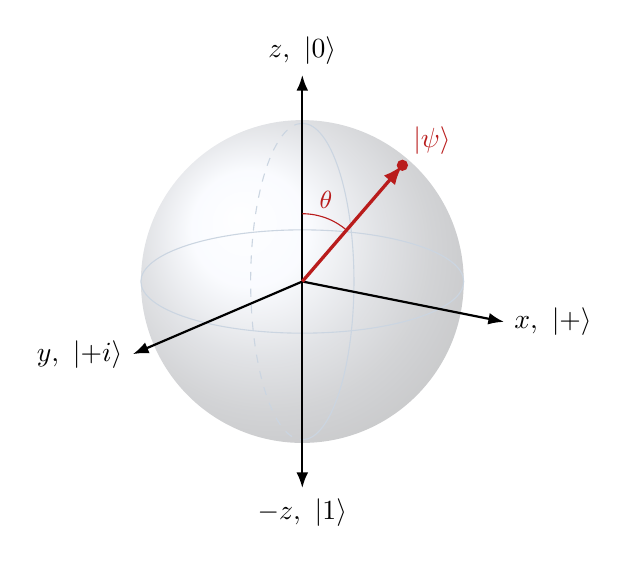
\begin{tikzpicture}[scale=2.05]
  \shade[ball color=QpuBlue!10,opacity=.32] (0,0) circle (1);
  \draw[QpuLine] (0,0) ellipse (1 and .32);
  \draw[QpuLine,dashed] (0,.98) arc (90:270:.32 and .98);
  \draw[QpuLine] (0,-.98) arc (-90:90:.32 and .98);
  \draw[-{Latex[length=2mm]},thick] (0,0)--(0,1.28) node[above] {$z,\ \ket0$};
  \draw[-{Latex[length=2mm]},thick] (0,0)--(0,-1.28) node[below] {$-z,\ \ket1$};
  \draw[-{Latex[length=2mm]},thick] (0,0)--(1.25,-.25) node[right] {$x,\ \ket+$};
  \draw[-{Latex[length=2mm]},thick] (0,0)--(-1.05,-.45) node[left] {$y,\ \ket{+i}$};
  \draw[-{Latex[length=2.5mm]},very thick,QpuRed] (0,0)--(.62,.72)
    node[above right] {$\ket{\psi}$};
  \draw[QpuRed] (0,.42) arc (90:49:.42) node[midway,above] {\small$\theta$};
  \fill[QpuRed] (.62,.72) circle (.035);
\end{tikzpicture}
\end{center}

The north pole is $\ket0$ and the south pole is $\ket1$. The equator contains
equal-magnitude superpositions. $\ket+$ points along $+x$,
$\ket-=(\ket0-\ket1)/\sqrt2$ along $-x$,
and $\ket{+i}=(\ket0+i\ket1)/\sqrt2$ along $+y$.

\subsection{How gates move a Bloch vector}

Ignoring global phase, many one-qubit gates are rotations:
\begin{itemize}
  \item X rotates the sphere by $\pi$ around the x-axis, exchanging north and
  south.
  \item Y rotates by $\pi$ around the y-axis.
  \item Z rotates by $\pi$ around the z-axis, changing relative phase.
  \item S and T rotate around z by $\pi/2$ and $\pi/4$.
  \item PHASE rotates around z by its supplied angle $\theta$.
  \item H rotates the coordinate description so the z basis and x basis are
  exchanged: $\ket0\leftrightarrow\ket+$ and
  $\ket1\leftrightarrow\ket-$.
\end{itemize}
The sphere is a teaching model for one pure qubit. It cannot display the full
state of entangled multi-qubit systems as one ordinary three-dimensional arrow.


\section{Multiple qubits and entanglement}

\subsection{Tensor products}

Two classical bits have four possibilities; two qubits have four basis vectors:
\[
\ket{00},\ \ket{01},\ \ket{10},\ \ket{11}.
\]
Independent systems combine with the tensor product $\otimes$. If
$\ket A=[a_0,a_1]^T$ and $\ket B=[b_0,b_1]^T$, then
\[
\ket A\otimes\ket B=
\begin{bmatrix}
a_0b_0\\a_0b_1\\a_1b_0\\a_1b_1
\end{bmatrix}.
\]
For $n$ qubits, the simulator stores $2^n$ amplitudes:
\[
\ket{\Psi}=\sum_{x=0}^{2^n-1}a_x\ket{x},\qquad
\sum_x|a_x|^2=1.
\]
This exponential growth is why state-vector simulation becomes expensive as
qubit count increases.

\subsection{Entanglement}

Some multi-qubit states cannot be factored into independent one-qubit states.
The Bell state
\[
\ket{\Phi^+}=\frac{\ket{00}+\ket{11}}{\sqrt2}
\]
is entangled. Each qubit measured alone is equally likely to be 0 or 1, but
their outcomes are perfectly correlated. It can be prepared from $\ket{00}$:
\begin{lstlisting}
H -I A -O A
CNOT -I A -O B
\end{lstlisting}
The first gate creates a superposition; the controlled gate correlates B with
A. Entanglement is not a classical alias. It is a property of the joint
amplitude vector.

\subsection{Controlled operations}

A controlled gate applies a target operation only on basis components where
its control condition is true. CNOT applies X when its control is one. If the
control is in superposition, linearity applies the operation to one branch and
not the other, which can create entanglement:
\[
\frac{\ket0+\ket1}{\sqrt2}\otimes\ket0
\xrightarrow{\mathrm{CNOT}}
\frac{\ket{00}+\ket{11}}{\sqrt2}.
\]
CCNOT requires both controls to be one. The system's OR and XOR derived gates
use ``any active'' and ``odd parity'' predicates respectively.


\section{Measurement, probability, and truth tables}

\subsection{Projective measurement}

For a measured qubit $q$ in a multi-qubit state,
\[
P(q=1)=\sum_{x:\,x_q=1}|a_x|^2,\qquad
P(q=0)=1-P(q=1).
\]
The simulator samples one outcome. Amplitudes incompatible with that outcome
become zero; compatible amplitudes are divided by the square root of the kept
probability so the state is normalized again. Measurement is destructive in
the sense that the pre-measurement superposition is generally unavailable
after collapse.

\subsection{Single runs and repeated runs}

One simulation run produces one measurement sample. To estimate a probability,
run the same preparation and circuit many times. If a plus state is measured
1 approximately 500 times in 1000 shots, the observed frequency $500/1000$
estimates the theoretical probability $1/2$. More shots reduce ordinary
sampling noise but never reveal a complex amplitude directly.

\subsection{Truth tables versus quantum amplitudes}

A classical truth table specifies output bits for listed input bits. It is a
good contract for arithmetic and reversible Boolean circuits operating on
computational-basis states. It cannot fully describe phase, interference,
entanglement, or a probability distribution.

The QPU truth-table runner prepares each input row, executes the circuit,
measures declared RETURNVALS, and compares those measured bits. In companion
\code{.qpuio} tables, cells are \code{0p}, \code{1p}, or \code{sp}. On an
expected output, \code{sp} means ``either measured bit is acceptable.'' Use
state equations and repeated experiments in addition to tables when a circuit's
purpose is genuinely quantum.

\subsection{A complete interference example}

Starting in zero, two Hadamards restore zero:
\[
\ket0\xrightarrow{H}\ket+
\xrightarrow{H}\ket0.
\]
Inserting Z changes the relative phase and changes the final answer:
\[
\ket0\xrightarrow{H}\ket+
\xrightarrow{Z}\ket-
\xrightarrow{H}\ket1.
\]
\begin{lstlisting}
MAIN-PROCESS Interference
CREATETOKEN -I Q
SET Q 0p
H -I Q -O Q
Z -I Q -O Q
H -I Q -O Q
MEASURE -I Q
RETURNVALS Q
\end{lstlisting}
The middle Z does not change an immediate 0/1 probability, yet interference at
the final H makes its effect deterministic. This is the central reason the
system documents matrices and phase as well as truth tables.


\section{Single-qubit primitive gates}

\GateHeading{Pauli X}{X}{\GateSegment{X}}

\[
X=\begin{bmatrix}0&1\\1&0\end{bmatrix},\quad
X\ket0=\ket1,\quad X\ket1=\ket0,\quad
X(\alpha\ket0+\beta\ket1)=\beta\ket0+\alpha\ket1.
\]
X is the quantum bit flip. On the Bloch sphere it is a half-turn around the
x-axis. It exchanges the north and south poles and is self-inverse:
$X^2=I$. Unlike a classical NOT implementation, X remains meaningful on a
superposition because it exchanges amplitudes linearly without measuring.
\begin{lstlisting}
X -I Q:0 -O Q:0
\end{lstlisting}
\begin{center}
\begin{tabular}{ccc}\toprule Input & Classical comparison & Output\\\midrule
0 & NOT 0 & 1\\
1 & NOT 1 & 0\\\bottomrule\end{tabular}
\end{center}

\GateHeading{Pauli Y}{Y}{\GateSegment{Y}}

\[
Y=\begin{bmatrix}0&-i\\i&0\end{bmatrix},\quad
Y\ket0=i\ket1,\quad Y\ket1=-i\ket0.
\]
It flips the basis value like X but adds phases that become observable through
later interference. Geometrically it is a half-turn around the y-axis and is
self-inverse, $Y^2=I$. The factors $i$ and $-i$ are global phases for either
basis state by itself, but on components of a larger superposition they may
become relative phases.
\begin{lstlisting}
Y -I Q -O Q
\end{lstlisting}
\begin{center}
\begin{tabular}{ccc}\toprule Input & Measured bit & Quantum output\\\midrule
0 & 1 & $i\ket1$\\
1 & 0 & $-i\ket0$\\\bottomrule\end{tabular}
\end{center}

\GateHeading{Pauli Z}{Z}{\GateSegment{Z}}

\[
Z=\begin{bmatrix}1&0\\0&-1\end{bmatrix},\quad
Z\ket0=\ket0,\quad Z\ket1=-\ket1.
\]
Z does not change a computational-basis measurement, but it changes relative
phase. For example, $Z\ket+=\ket-=(\ket0-\ket1)/\sqrt2$.
On the Bloch sphere it is a half-turn around z. It is self-inverse and is the
simplest example showing why quantum state cannot be reduced to a table of
immediate measurement probabilities.
\begin{lstlisting}
Z -I Q -O Q
\end{lstlisting}
\begin{center}
\begin{tabular}{ccc}\toprule Input & Classical bit & Quantum output\\\midrule
0 & 0 & $\ket0$\\
1 & 1 & $-\ket1$\\\bottomrule\end{tabular}
\end{center}

\GateHeading{Hadamard}{H}{\GateSegment{H}}

\[
H=\frac1{\sqrt2}\begin{bmatrix}1&1\\1&-1\end{bmatrix},\quad
H\ket0=\ket+,\quad H\ket1=\ket-.
\]
Hadamard changes between the computational z basis and the plus/minus x basis.
It creates equal magnitudes from a basis state, but the sign of the second
amplitude depends on the input. It is also self-inverse: applying H twice
returns the original state. H is commonly used before controlled gates to
create entanglement and after phase gates to reveal interference.
\begin{lstlisting}
SET Q 0p
H -I Q -O Q
MEASURE -I Q
\end{lstlisting}
\begin{center}
\begin{tabular}{ccc}\toprule Input & Measurement distribution & State before measurement\\\midrule
0 & 50\% 0, 50\% 1 & $(\ket0+\ket1)/\sqrt2$\\
1 & 50\% 0, 50\% 1 & $(\ket0-\ket1)/\sqrt2$\\\bottomrule\end{tabular}
\end{center}
Equal classical probabilities hide the relative minus sign responsible for
interference.

\GateHeading{S phase}{S}{\GateSegment{S}}

\[
S=P(\pi/2)=\begin{bmatrix}1&0\\0&i\end{bmatrix},\qquad
S\ket1=i\ket1,\qquad S^2=Z.
\]
S is a quarter-turn around the Bloch sphere's z-axis. It changes $\ket+$ into
$(\ket0+i\ket1)/\sqrt2$ while leaving basis measurement probabilities
unchanged. Its inverse is $S^\dagger=P(-\pi/2)$, not S itself.
\begin{lstlisting}
S -I Q -O Q
\end{lstlisting}
\begin{center}
\begin{tabular}{ccc}\toprule Input & Measured bit & Quantum output\\\midrule
0 & 0 & $\ket0$\\
1 & 1 & $i\ket1$\\\bottomrule\end{tabular}
\end{center}

\GateHeading{T phase}{T}{\GateSegment{T}}

\[
T=P(\pi/4)=\begin{bmatrix}1&0\\0&e^{i\pi/4}\end{bmatrix},\qquad
T^2=S,\qquad T^4=Z.
\]
T is an eighth-turn around z. Together with gates such as H and CNOT, it is an
important non-Clifford resource for expressing general quantum computations.
Its inverse is $T^\dagger=P(-\pi/4)$; the current \code{BT} spelling does not
synthesize that inverse, so use \code{BPHASE=pi/4} when the negative phase is
required.
\begin{lstlisting}
T -I Q -O Q
\end{lstlisting}
\begin{center}
\begin{tabular}{ccc}\toprule Input & Measured bit & Quantum output\\\midrule
0 & 0 & $\ket0$\\
1 & 1 & $e^{i\pi/4}\ket1$\\\bottomrule\end{tabular}
\end{center}

\GateHeading{Arbitrary phase}{PHASE}{\GateSegment{$P(\theta)$}}

\[
P(\theta)=\begin{bmatrix}1&0\\0&e^{i\theta}\end{bmatrix},\qquad
\alpha\ket0+\beta\ket1\mapsto
\alpha\ket0+\beta e^{i\theta}\ket1.
\]
PHASE is the general form behind S, T, and Z. It preserves
$|\alpha|^2$ and $|\beta|^2$ because $|e^{i\theta}|=1$, yet rotates the
relative phase by $\theta$. On the Bloch sphere this is a z-axis rotation up to
global phase. A later H or another basis-changing gate is normally needed to
turn that phase difference into changed computational-basis probabilities.
The angle is embedded in the opcode:
\begin{lstlisting}
PHASE=1.5708 -I Q -O Q     # radians
PHASE=3/2 -I Q -O Q        # rational radians
PHASE=90d -I Q -O Q        # degrees
PHASE=45/2d -I Q -O Q      # rational degrees
PHASE=pi -I Q -O Q
PHASE=-11pi/6 -I Q -O Q
PHASE=2*pi/3 -I Q -O Q
BPHASE=pi/4 -I Q -O Q      # P(-pi/4)
\end{lstlisting}
Accepted numeric atoms include signed integers, decimals, leading-dot decimals,
and one optional rational denominator. Pi notation accepts an optional sign,
an integer coefficient, an optional \code{*}, and an optional positive integer
denominator. A zero denominator and malformed angle raise an error.

\begin{center}
\begin{tabular}{ccc}\toprule Input & Measured bit & Quantum output\\\midrule
0 & 0 & $\ket0$\\
1 & 1 & $e^{i\theta}\ket1$\\\bottomrule\end{tabular}
\end{center}

\subsection{Backward-prefix syntax}

The QPU language recognizes a leading \code{B} before a supported primitive gate name,
for example \code{BX}, \code{BH}, \code{BCNOT}, or \code{BSWAP}, and sets
\code{reverse=true}. (Compiler-internal \code{RESET} remains unavailable in
source.) Only \code{BPHASE=angle} currently changes emitted behavior: the
compiler negates the phase angle. For every other gate the flag is metadata
only. Emitting the ordinary gate still gives the mathematical inverse for these
self-inverse gates:
\[
X,\ Y,\ Z,\ H,\ \mathrm{CNOT},\ \mathrm{CCNOT},\
\mathrm{CZ},\ \mathrm{CY},\ \mathrm{SWAP}.
\]
In contrast, \code{BS} and \code{BT} do not synthesize $S^\dagger$ or
$T^\dagger$. Do not rely on B-prefixed forms for inverse execution unless the
gate is self-inverse or is \code{BPHASE}.


\section{Controlled and two-qubit primitive gates}

\GateHeading{Controlled NOT}{CNOT}{\ControlledSegment{$\oplus$}}

\[
\ket{c,t}\longmapsto\ket{c,t\oplus c}.
\]
CNOT leaves the control unchanged. When the control is zero, the target is
unchanged; when the control is one, X acts on the target. Because the map is a
permutation of basis states, it is reversible and self-inverse. A
superposition control can entangle the wires, so ``classical XOR'' describes
only its basis-state action.
\begin{lstlisting}
CNOT -I Control -O Target
\end{lstlisting}
\begin{center}
\begin{tabular}{cc|cc}\toprule $c$&$t$&$c'$&$t'$\\\midrule
0&0&0&0\\0&1&0&1\\1&0&1&1\\1&1&1&0\\\bottomrule
\end{tabular}
\end{center}
CNOT is a reversible embedding of XOR because it preserves the control.
In the workbench, the control comes from \textbf{Control A} and the target
from \textbf{Target particle}; \textbf{Control B} is ignored.

\GateHeading{Doubly controlled NOT / Toffoli}{CCNOT}{\DoubleControlledSegment}

\[
\ket{a,b,t}\longmapsto\ket{a,b,t\oplus(a\land b)}.
\]
CCNOT, also called Toffoli, applies X only when both controls are one. It is a
reversible universal building block for classical computation embedded in a
quantum circuit. The target's previous value matters: zero computes AND, while
one computes NAND. The gate is self-inverse.
\begin{lstlisting}
CCNOT -I A B -O Target
\end{lstlisting}
\begin{center}
\begin{tabular}{ccc|ccc}\toprule $a$&$b$&$t$&$a'$&$b'$&$t'$\\\midrule
0&0&0&0&0&0\\0&0&1&0&0&1\\
0&1&0&0&1&0\\0&1&1&0&1&1\\
1&0&0&1&0&0\\1&0&1&1&0&1\\
1&1&0&1&1&1\\1&1&1&1&1&0\\\bottomrule
\end{tabular}
\end{center}
With a target initialized to zero, Toffoli computes classical AND reversibly.

\begin{beginnerbox}[Controls are preserved, the target is the output]
In the table, the $a'$ and $b'$ columns always equal $a$ and $b$: the two
controls are only read. Only $t$ can change, and it flips exactly in the two
rows where $a=b=1$. In the \textbf{Interactive workbench}, choose
\textbf{CCNOT} in \textbf{Gate}, the two inputs in \textbf{Control A} and
\textbf{Control B}, and the output wire in \textbf{Target particle}. The
\emph{CCNOT demo} starter circuit is exactly this gate with both controls
prepared as 1.
\end{beginnerbox}

\GateHeading{Controlled Z}{CZ}{\ControlledSegment{Z}}

\[
\mathrm{CZ}\ket{c,t}=(-1)^{ct}\ket{c,t},\qquad
\mathrm{CZ}=\operatorname{diag}(1,1,1,-1).
\]
CZ adds a minus sign only to the $\ket{11}$ amplitude. No computational-basis
bit changes, but superpositions can acquire observable relative phase. CZ is
symmetric between its two wires, even though QPU syntax writes one as the
input control and one as the output target. It is self-inverse.
\begin{lstlisting}
CZ -I Control -O Target
\end{lstlisting}
\begin{center}
\begin{tabular}{cc|cc}\toprule Input & Measured output & Amplitude multiplier & State\\\midrule
00&00&$+1$&$\ket{00}$\\01&01&$+1$&$\ket{01}$\\
10&10&$+1$&$\ket{10}$\\11&11&$-1$&$-\ket{11}$\\\bottomrule
\end{tabular}
\end{center}
The classical columns are unchanged; the quantum phase is the operation.

\GateHeading{Controlled phase}{CPHASE}{\ControlledSegment{$P(\theta)$}}

\[
\ket{11}\longmapsto e^{i\theta}\ket{11},
\]
while $\ket{00}$, $\ket{01}$, and $\ket{10}$ are unchanged. CZ is the special
case $\theta=\pi$. CPHASE unlocks compact Quantum Fourier Transform and
phase-estimation demos.
\begin{lstlisting}
CPHASE=pi/2 -I Control -O Target
CPHASE=90d -I Control -O Target
\end{lstlisting}

\GateHeading{Controlled Y}{CY}{\ControlledSegment{Y}}

\[
\ket{0,t}\mapsto\ket{0,t},\quad
\ket{1,0}\mapsto i\ket{1,1},\quad
\ket{1,1}\mapsto-i\ket{1,0}.
\]
CY applies the Pauli Y rotation to the target only when the control is one. Its
basis-bit pattern resembles CNOT, but the $\pm i$ factors distinguish their
behavior on superpositions. Since $Y^2=I$, CY is self-inverse.
\begin{lstlisting}
CY -I Control -O Target
\end{lstlisting}
\begin{center}
\begin{tabular}{cc|cc|c}\toprule $c$&$t$&$c'$&$t'$&Quantum phase\\\midrule
0&0&0&0&$+1$\\0&1&0&1&$+1$\\
1&0&1&1&$i$\\1&1&1&0&$-i$\\\bottomrule
\end{tabular}
\end{center}

\GateHeading{Swap}{SWAP}{\SwapSegment}

\[
\mathrm{SWAP}\ket{a,b}=\ket{b,a}.
\]
SWAP exchanges the complete quantum states of two wires, including amplitudes
and any correlations with the rest of the register. It does not copy either
state. Three CNOTs can decompose SWAP, but the QPU system provides it as one
primitive instruction. Applying SWAP twice restores the original ordering.
\begin{lstlisting}
SWAP -I A B -O A B
\end{lstlisting}
The two output tokens are mandatory and must resolve to the same two wires, in
the same order, as the inputs.
\begin{center}
\begin{tabular}{cc|cc}\toprule $a$&$b$&$a'$&$b'$\\\midrule
0&0&0&0\\0&1&1&0\\1&0&0&1\\1&1&1&1\\\bottomrule
\end{tabular}
\end{center}


\section{Derived logical gates}

Derived gates are QPU instructions implemented as reversible target
mutations. Inputs are preserved. If target $t$ starts in zero, AND/OR/XOR
write the familiar classical function. If it does not, the true behavior is
the XOR embedding shown below.

\begin{beginnerbox}[One shape for every two-input gate]
AND, NAND, OR, and XOR all follow $t' = t\oplus f(a,b)$. The two inputs $a$
and $b$ (\textbf{Control A} and \textbf{Control B} in the workbench) are read
and left unchanged. The target $t$ (\textbf{Target particle}) is the output
workspace and is the only wire that changes. Only $f$ differs between the
four gates. To get the ordinary classical answer, start the target at 0 with
\code{SET Out 0p}.
\end{beginnerbox}

\GateHeading{Logical NOT}{NOT}{\GateSegment{$\neg$}}

\[
t'\;=\;t\oplus1.
\]
NOT is the derived logical spelling of a bit flip. In the current simulator it
uses the same X matrix on the output target. The required input establishes the
one-input instruction shape, but a distinct input is not copied into the
output; use the same token on both sides.
\begin{lstlisting}
NOT -I Target -O Target
\end{lstlisting}
\begin{center}
\begin{tabular}{c|c}\toprule $t$&$t'$\\\midrule0&1\\1&0\\\bottomrule\end{tabular}
\end{center}
The current gate implementation mutates the output target. Use the same token
for input and output; a distinct input token is not copied.

\GateHeading{Reversible AND}{AND}{\DoubleControlledSegment}

\[
t'=t\oplus(a\land b).
\]
AND flips the target exactly on the basis components where both controls are
one. This is Toffoli-style behavior. It remains linear on superpositions and
may entangle the target with its controls. Calling it AND is convenient only
when the target is deliberately initialized.
\begin{lstlisting}
SET Out 0p
AND -I A B -O Out
\end{lstlisting}
\begin{center}
\begin{tabular}{cc|c|c}\toprule $a$&$b$&$t=0$&$t'=a\land b$\\\midrule
0&0&0&0\\0&1&0&0\\1&0&0&0\\1&1&0&1\\\bottomrule
\end{tabular}
\end{center}

\GateHeading{Reversible NAND}{NAND}{\DoubleControlledSegment}

\[
t'=t\oplus(a\land b)\oplus1.
\]
NAND first performs the all-controls-active mutation and then inverts the
target. With target zero it produces the familiar NAND column. With target one
it instead produces AND, illustrating why reversible target state must always
be included in the full mathematical definition.
\begin{lstlisting}
SET Out 0p
NAND -I A B -O Out
\end{lstlisting}
\begin{center}
\begin{tabular}{cc|c|c}\toprule $a$&$b$&$t=0$&$t'=\neg(a\land b)$\\\midrule
0&0&0&1\\0&1&0&1\\1&0&0&1\\1&1&0&0\\\bottomrule
\end{tabular}
\end{center}

\GateHeading{Reversible OR}{OR}{\DoubleControlledSegment}

\[
t'=t\oplus(a\lor b).
\]
OR uses an ``any control is one'' predicate. If either or both controls are
active, the target is flipped. This direct derived operation is equivalent on
basis states to combining XOR and AND through
$a\lor b=a\oplus b\oplus(a\land b)$.
\begin{lstlisting}
SET Out 0p
OR -I A B -O Out
\end{lstlisting}
\begin{center}
\begin{tabular}{cc|c|c}\toprule $a$&$b$&$t=0$&$t'=a\lor b$\\\midrule
0&0&0&0\\0&1&0&1\\1&0&0&1\\1&1&0&1\\\bottomrule
\end{tabular}
\end{center}
For bits, $a\lor b=a\oplus b\oplus(a\land b)$.

\GateHeading{Reversible XOR}{XOR}{\DoubleControlledSegment}

\[
t'=t\oplus a\oplus b.
\]
XOR flips the target when an odd number of controls is one. With two inputs,
this is the ordinary exclusive-or predicate. The parity definition explains
why the 11 row does not flip: two active controls have even parity.
\begin{lstlisting}
SET Out 0p
XOR -I A B -O Out
\end{lstlisting}
\begin{center}
\begin{tabular}{cc|c|c}\toprule $a$&$b$&$t=0$&$t'=a\oplus b$\\\midrule
0&0&0&0\\0&1&0&1\\1&0&0&1\\1&1&0&0\\\bottomrule
\end{tabular}
\end{center}


\section{Measurement gate}

\GateHeading{Measurement}{MEASURE}{\MeasureSegment}

\begin{lstlisting}
MEASURE -I Q     # exactly one named wire
MEASURE          # every wire known at this point
\end{lstlisting}
\code{MEASURE} takes no \code{-O}. Repeated one-wire commands are useful when
only declared returns should become classical. A bare command emits one
measurement operation per currently allocated wire.

\begin{center}
\begin{tabular}{c|c|c}\toprule State & Outcome probabilities & Collapsed state\\\midrule
$\ket0$ & $P(0)=1$ & $\ket0$\\
$\ket1$ & $P(1)=1$ & $\ket1$\\
$\alpha\ket0+\beta\ket1$ & $P(0)=|\alpha|^2$, $P(1)=|\beta|^2$ &
$\ket0$ or $\ket1$\\\bottomrule
\end{tabular}
\end{center}


\section{Reset: an operation that is not a gate}
\hypertarget{reset-semantics}{}

The word \emph{reset} appears in two unrelated places: the compiler's internal
\code{RESET} operation, and three buttons in the Circuit builder. Neither is an
ordinary quantum gate.

\subsection{Reversible gates versus RESET}

Every gate in the palette except the meter is \emph{reversible}: its effect
can always be undone. X, Y, Z, H, CNOT, CCNOT, CZ, CY, SWAP, NOT, AND, NAND,
OR, and XOR undo themselves when applied a second time. S, T, and PHASE are
undone by the same phase with the opposite sign. Mathematically each is a
\emph{unitary} matrix $U$, and $U^\dagger$ undoes it.

\code{RESET} is different. It forces one wire to $\ket0$ whatever it held
before:
\[
\ket0\mapsto\ket0,\qquad \ket1\mapsto\ket0,\qquad
\alpha\ket0+\beta\ket1\mapsto\ket0 .
\]
Two different inputs, $\ket0$ and $\ket1$, give the same output, so nothing
can tell afterwards which one was there. The information has been erased, and
no matrix $U$ can undo that. RESET is therefore not unitary, just like
MEASURE.

\begin{center}
\begin{tabularx}{\textwidth}{>{\bfseries}l X X X}
\toprule
& Reversible gates (X, H, CNOT, AND, \ldots) & MEASURE & RESET\\
\midrule
Unitary? & Yes & No & No\\
Can be undone? & Yes, by the inverse gate & No & No\\
Result depends on chance? & No & Yes & No\\
Written in source? & Yes & Yes & No --- write \code{SET wire 0p}\\
Shown on canvas? & Yes & Yes, as the meter & No (hidden)\\
\bottomrule
\end{tabularx}
\end{center}

\subsection{Where RESET comes from}

You never type RESET. The compiler inserts it when a wire must start at zero:
\begin{itemize}
  \item \code{SET Out 0p} on a workspace wire. (\code{SET Out 1p} and
  \code{SET Out sp} are instead prepared by applying X or H to a wire that
  starts at 0.)
  \item \code{INCREASECYCLE}, which zeroes pending workspace before the next
  stage.
  \item \code{RUNCHILD} and \code{CALL}, which zero each parent output wire
  once before expanding the child.
\end{itemize}
RESET steps are hidden from the canvas and filtered from the
\textbf{Execution log} so that the visible circuit shows only the gates you
wrote. They still run during simulation.

\begin{cautionbox}[Reset a wire only when it is not entangled]
In this simulator, RESET keeps the part of the state in which the wire is
already 0 and rescales it; only if that part is empty does it move the
$\ket1$ amplitudes to $\ket0$. On a fresh wire this is exactly ``prepare
$\ket0$''. On a wire entangled with others it also changes the other wires.
For example, resetting one half of a Bell pair forces the other half to 0 as
well. In multi-stage circuits, \emph{uncompute} temporary wires back to 0 with
reversible gates instead of relying on a reset.
\end{cautionbox}

\subsection{Reset buttons compared}
\hypertarget{reset-buttons}{}

None of these buttons inserts a RESET operation into your circuit. They only
change what the page is showing and simulating.

\begin{center}
\begin{tabularx}{\textwidth}{>{\raggedright\arraybackslash}p{0.2\textwidth}>{\centering\arraybackslash}p{0.13\textwidth}>{\centering\arraybackslash}p{0.13\textwidth}>{\centering\arraybackslash}p{0.13\textwidth}X}
\toprule
Kept or cleared? & \textbf{Reset state} & \textbf{Clear circuit} & \textbf{Reset site} & Notes\\
\midrule
Gates on the canvas & kept & cleared & cleared & \\
Number of wires & kept & kept & back to 3 & \\
Start states (\emph{name} start) & kept & kept & all \code{0p} & \\
Protocol editor text & kept & rewritten & default & Clear circuit writes an
empty canvas protocol into the editor.\\
Compiled PARAMS / RETURNVALS & kept & cleared & cleared & \\
Quantum state and measurements & rewound & rewound & rewound & Back to the
start states; log restarts.\\
Workbench selections & kept & kept & defaults & Gate H, target q0, controls
q1 and q2, phase 90\textdegree.\\
Custom gates and catalog & kept & kept & kept & Nothing removes these except
\textbf{Remove} or closing the browser session.\\
\bottomrule
\end{tabularx}
\end{center}

\begin{beginnerbox}[Which one do I want?]
\begin{description}
  \item[Reset state] ``Run the same experiment again.'' Use it between
  repeated runs of a circuit that measures, to collect several samples.
  \item[Clear circuit] ``Keep my wires, start a new circuit.''
  \item[Reset site] ``Put everything back the way it was when I first opened
  the page.'' The \textbf{Reset site} entry in the navigation menu and
  \textbf{Reset site completely} on the \textbf{More} page do the same thing.
\end{description}
\end{beginnerbox}

\section{Mixed states, entanglement measures, and noise}
\hypertarget{mixed-states}{}

Every simulation in QPU passes through one \emph{physics engine}. The compiler
turns source into gates and the simulator decides the order in which they run,
but the physics engine alone changes the quantum state and computes the
quantities in this chapter. The particle cards in the Circuit builder show
several of them.

\subsection{Density matrices}

A pure state $\ket\psi$ can also be written as the \emph{density matrix}
\[
\rho=\ket\psi\bra\psi,\qquad \rho_{ij}=a_i\,\overline{a_j}.
\]
The diagonal entries are the basis probabilities. The off-diagonal entries,
called \emph{coherences}, carry the relative phases that make interference
possible. A \emph{mixed state} is a weighted mixture of pure states,
\[
\rho=\sum_k p_k\ket{\psi_k}\bra{\psi_k},\qquad p_k\ge0,\quad \sum_k p_k=1,
\]
and describes either classical uncertainty about which state was prepared or a
part of a larger entangled system. Every density matrix is Hermitian, has
trace 1, and has no negative eigenvalues. Global phase cancels in
$\ket\psi\bra\psi$, so a density matrix records exactly the physically
observable part of a state.

\subsection{Reduced states and the partial trace}

A single wire of an entangled register has no state vector of its own, but it
always has a density matrix. For a system $AB$ the state of $A$ alone is the
\emph{partial trace}
\[
\rho_A=\operatorname{Tr}_B(\rho_{AB}),\qquad
(\rho_A)_{ij}=\sum_{k}(\rho_{AB})_{(i,k),(j,k)}.
\]
It gives the correct statistics for every measurement made on $A$ alone. For
one qubit it fixes a \emph{Bloch vector} $(x,y,z)$ through
\[
\rho=\tfrac12\left(I+xX+yY+zZ\right),\qquad
x=\langle X\rangle,\quad y=\langle Y\rangle,\quad z=\langle Z\rangle.
\]
Pure states lie on the Bloch sphere ($r=1$); mixed states lie inside the
Bloch ball ($r<1$). The particle cards draw each wire from its reduced state,
which is why an entangled wire's arrow shrinks toward the centre.

\subsection{Purity and mixedness}

The purity of a state is
\[
P=\operatorname{Tr}(\rho^2)=\sum_{ij}|\rho_{ij}|^2 .
\]
$P=1$ exactly for pure states. For one qubit $P=(1+r^2)/2$, which ranges from
1 on the sphere to $\tfrac12$ at the centre (the maximally mixed state $I/2$).
The particle card's \emph{mixedness} is the normalized linear entropy
$M=2(1-P)$: 0 for a pure wire and 1 for a maximally mixed one.

\begin{beginnerbox}[Mixed does not mean noisy]
Without noise, the whole register is always in a pure state. A wire can still
look mixed because it is entangled with other wires: its information lives in
the correlations, not in the wire alone. When the register is pure and a wire
is mixed, the card shows \textbf{Entangled with register}.
\end{beginnerbox}

\subsection{Entropy and entanglement}

The \emph{von Neumann entropy} measures how mixed a state is, in bits:
\[
S(\rho)=-\operatorname{Tr}(\rho\log_2\rho)=-\sum_k\lambda_k\log_2\lambda_k,
\]
where $\lambda_k$ are the eigenvalues of $\rho$. A pure state has $S=0$; a
maximally mixed qubit has $S=1$.

If the whole register is pure, a subsystem $A$ is entangled with the rest
exactly when $\rho_A$ is mixed, and $S(\rho_A)$ is the \emph{entanglement
entropy}: how many bits of entanglement join $A$ to the rest.

\begin{center}
\begin{tabularx}{\textwidth}{l X X X}
\toprule
State & One qubit & Two qubits together & Whole register\\
\midrule
$\ket{00}$ & $P=1$, $S=0$ & $P=1$ & pure\\
Bell $(\ket{00}+\ket{11})/\sqrt2$ & $P=\tfrac12$, $S=1$ & $P=1$ & pure\\
GHZ $(\ket{000}+\ket{111})/\sqrt2$ & $P=\tfrac12$, $S=1$ & $P=\tfrac12$, $S=1$ & pure\\
\bottomrule
\end{tabularx}
\end{center}

The GHZ row shows why entanglement cannot be reduced to pairwise links. Any
two GHZ qubits are only classically correlated (00 or 11 with equal chance),
yet all three together form a single pure, entangled state. Questions about
entanglement are therefore always about a chosen split of the register into a
subsystem and the rest.

When the whole register is mixed, for example after noise, local mixedness no
longer proves entanglement. The physics engine then uses the \emph{partial
transpose} test: transpose only $B$'s indices of $\rho_{AB}$. If the result
has a negative eigenvalue the state is entangled, and the sum of the negative
eigenvalues' magnitudes is the \emph{negativity} ($\tfrac12$ for a Bell pair).
A negative eigenvalue is proof for any split. The converse holds only for two
qubits (or a qubit and a qutrit): for larger splits some entangled states have
no negative eigenvalue at all. The engine therefore reports one of three
results, and says which test it used:

\begin{center}
\begin{tabularx}{\textwidth}{l X}
\toprule
Result & Meaning\\
\midrule
entangled & Proven: the reduced state of a pure register is mixed, or the
partial transpose has a negative eigenvalue.\\
separable & Proven: the reduced state of a pure register is pure, or a
two-qubit mixed state has no negative eigenvalue.\\
inconclusive & Not decided: a larger mixed split passed the partial-transpose
test, or the register is too large to test. This is \emph{not} evidence that
the wires are unentangled.\\
\bottomrule
\end{tabularx}
\end{center}
A particle card shows \textbf{Entangled with register} only for a proven
result and \textbf{Entanglement undetermined} for an inconclusive one; it
never labels a wire ``not entangled'' because a test failed to find
entanglement.

QPU has no \code{ENTANGLE} instruction. Entanglement always comes from
ordinary gates such as \code{H} followed by \code{CNOT}; the physics engine
only detects and measures it.

\subsection{Measurement in other bases}

\code{MEASURE} measures in the computational (Z) basis. The physics engine can
also measure the X and Y observables by rotating the wire's eigenbasis onto Z,
measuring, and rotating back:
\begin{center}
\begin{tabular}{llll}
\toprule
Basis & Outcome 0 & Outcome 1 & Rotation onto Z\\
\midrule
Z & $\ket0$ & $\ket1$ & none\\
X & $\ket+$ & $\ket-$ & $H$\\
Y & $\ket{+i}$ & $\ket{-i}$ & $HS^\dagger$\\
\bottomrule
\end{tabular}
\end{center}
The state $\ket+$ gives a random result in the Z basis but always gives 0 in
the X basis: what a measurement reveals depends on the observable. In QPU
source, \code{MEASURE -I Q -BASIS X} (or \code{Y}) chooses the observable; a
\code{MEASURE} without \code{-BASIS} is a Z measurement.

\subsection{Fidelity}

\emph{Fidelity} measures how close a simulated state $\rho$ is to an intended
state $\sigma$:
\[
F(\rho,\sigma)=\left(\operatorname{Tr}\sqrt{\sqrt\rho\,\sigma\sqrt\rho}\right)^2,
\qquad
F(\ket\psi,\ket\phi)=|\langle\psi|\phi\rangle|^2 .
\]
$F=1$ means the states are identical (up to global phase) and $F=0$ means they
are perfectly distinguishable. For example, $F(\ket+,\ket0)=\tfrac12$.

\subsection{Reset as a physical operation}

RESET forces a wire to $\ket0$. As a density-matrix operation it is the
\emph{reset channel}: the wire ends in $\ket0$ and whatever it shared with the
other wires is traced out,
\[
\rho\;\longmapsto\;\ket0\bra0\otimes\operatorname{Tr}_q(\rho).
\]
A state vector cannot hold the mixed result of resetting an entangled wire,
so a state-vector simulation follows one run of this channel the way real
hardware does: measure the wire in Z, then apply X if the result was 1.
Averaged over many runs this gives exactly the reset channel. The
\hyperlink{reset-semantics}{Reset} chapter describes what this means for
circuits.

\subsection{Noise and decoherence}

Real qubits are not isolated. Their interaction with the environment is
described by \emph{quantum channels}
\[
\rho\;\longmapsto\;\sum_k K_k\,\rho\,K_k^\dagger,
\qquad \sum_k K_k^\dagger K_k=I,
\]
which turn pure states into mixed ones. The physics engine provides these
single-qubit channels:
\begin{center}
\begin{tabularx}{\textwidth}{l X}
\toprule
Channel & Effect\\
\midrule
Bit flip ($p$) & $\rho\mapsto(1-p)\rho+pX\rho X$: $\ket0$ and $\ket1$ swap with probability $p$.\\
Phase flip ($p$) & $\rho\mapsto(1-p)\rho+pZ\rho Z$: coherences shrink by $1-2p$.\\
Depolarizing ($p$) & $\rho\mapsto(1-p)\rho+p\,I/2$: the Bloch vector shrinks by $1-p$.\\
Amplitude damping ($\gamma$) & Energy loss: $\ket1$ decays to $\ket0$ with probability $\gamma$.\\
Phase damping ($\lambda$) & Coherences shrink by $\sqrt{1-\lambda}$; populations are unchanged.\\
\bottomrule
\end{tabularx}
\end{center}

\emph{Decoherence} is usually quoted as two times. $T_1$ is the relaxation
time: after time $t$ an excited qubit remains in $\ket1$ with probability
$e^{-t/T_1}$. $T_2$ is the coherence time: off-diagonal entries decay as
$e^{-t/T_2}$. Physics requires $T_2\le2T_1$.

\begin{cautionbox}[Cycles are not time]
QPU cycles (\code{INCREASECYCLE}) are logical program stages, not elapsed
physical time. Decoherence uses a separate timing model that assigns a
duration to each gate. Noise is always optional: ordinary runs are ideal and
use the cheaper state vector ($2^n$ amplitudes) rather than a density matrix
($4^n$ entries). Choose \textbf{Run with noise} in the \textbf{Physics
inspector} on the Particle visualization page to rerun a circuit with a noise
channel and optional $T_1$/$T_2$; the inspector reports the fidelity with the
ideal run. Noise settings are not part of QPU source.
\end{cautionbox}

\subsection{No cloning and teleportation}

CNOT copies a known basis value onto a $\ket0$ target, but applied to
$\ket+\ket0$ it produces a Bell pair, not $\ket+\ket+$. The two results have
fidelity $\tfrac12$ and the target becomes entangled rather than a copy. This
is the \emph{no-cloning theorem}: no operation can copy an unknown quantum
state.

Quantum state can still be \emph{moved}. SWAP exchanges two wires' states, and
teleportation transfers a state using only ordinary operations: share a Bell
pair (\code{H}, \code{CNOT}), entangle the message with one half (\code{CNOT},
\code{H}), measure two wires, and apply \code{X} and \code{Z} to the
destination under classical \code{-IF} conditions. The destination then holds
the original state with fidelity 1 and the source wire has been measured, so
the state was never in two places at once. QPU has no \code{CLONE} or
\code{TELEPORT} instruction.

\section{Energy, frequency, and control pulses}
\hypertarget{frequency-and-pulses}{}

Gates in QPU are normally exact matrices. Real qubits are physical two-level
systems with an energy gap, and gates are made by driving them with
microwave pulses. The physics engine can model this level of detail. Frequency
is never a free display value: it is derived from each qubit's energy levels
and it drives the evolution.

Frequencies below are in GHz and times in ns, so $2\pi f t$ is a plain
angle. Energies use SI units.

\subsection{Energy levels and the Planck--Einstein relation}

A photon of frequency $f$ carries energy $E=hf=\hbar\omega$ with
$\omega=2\pi f$. A qubit absorbs or emits such a photon when it moves between
its levels, so its \emph{transition frequency} is
\[
f_{01}=\frac{E_1-E_0}{h}.
\]
The engine gives each modelled wire the idle Hamiltonian
\[
H_0=-\frac{\hbar\omega_{01}}{2}Z,
\]
whose levels are $E_0=-\hbar\omega_{01}/2$ and $E_1=+\hbar\omega_{01}/2$, a gap
of exactly $\hbar\omega_{01}$. A typical superconducting qubit at
$f_{01}=5$~GHz has $\Delta E\approx3.3\times10^{-24}$~J (about 21~$\mu$eV), and
the matching photon has a wavelength of about 6~cm.

\subsection{Free precession and the physical clock}

A qubit left alone still evolves: $e^{-iH_0t/\hbar}$ gives $\ket1$ a phase
relative to $\ket0$ that changes as
\[
\Delta\phi=-\omega_{01}\,\Delta t,
\]
so the Bloch vector precesses about the z-axis at $f_{01}$. Populations do not
change, which is why idle precession is invisible to Z measurements but
matters for everything that depends on relative phase.

Physical simulation keeps a \emph{physical clock}. Every operation lasts its
physical duration, and during that time every wire evolves under its own
Hamiltonian while $T_1$ and $T_2$ act over the same $\Delta t$. Logical cycles
(\code{INCREASECYCLE}) never advance this clock.

\subsection{Frames}

At several GHz the lab-frame phase turns billions of times a second. Most
calculations therefore use a \emph{rotating frame} that turns at each qubit's
nominal $f_{01}$. In that frame a perfectly calibrated idle qubit does
nothing, and only errors remain. A \code{frequencyOffset} (calibration error)
or a \code{frequencyDriftRate} (slow drift) leaves a residual precession
\[
\Delta\phi=-2\pi\!\int\!\bigl(f_{\mathrm{actual}}(t)-f_{\mathrm{nominal}}\bigr)\,dt,
\]
which becomes phase error in the circuit. The lab frame shows the full
precession.

\subsection{Driving a qubit: resonance, Rabi, and detuning}

A microwave drive of carrier frequency $\omega_d$ adds
\[
H_d(t)=\hbar\Omega(t)\cos(\omega_d t-\varphi)\,X,
\]
where $\Omega$ is the Rabi frequency, set by the drive amplitude, and $\varphi$
is the drive phase. In the frame rotating with the drive, the fast terms
average out and
\[
H\approx\frac{\hbar}{2}\bigl(\Delta Z+\Omega(\cos\varphi\,X+\sin\varphi\,Y)\bigr),
\qquad \Delta=\omega_d-\omega_{01}.
\]
\begin{itemize}
  \item \textbf{Resonance ($\Delta=0$).} The qubit rotates about an axis in
  the XY plane at the Rabi frequency, and the rotation angle is
  $\theta=\Omega t$ for a square pulse. A \emph{$\pi$-pulse}
  ($\Omega t=\pi$, $\varphi=0$) is an X gate up to global phase, and
  $\varphi=\pi/2$ gives Y. Starting from $\ket0$, $P(1)=\sin^2(\Omega t/2)$:
  these are \emph{Rabi oscillations}.
  \item \textbf{Detuning ($\Delta\neq0$).} The axis tilts toward z and the
  rotation speeds up to the \emph{generalized Rabi frequency}
  $\Omega'=\sqrt{\Omega^2+\Delta^2}$. Starting from $\ket0$,
  \[
  P(1)=\frac{\Omega^2}{\Omega^2+\Delta^2}\sin^2\!\frac{\Omega' t}{2},
  \]
  so a detuned drive never completes the flip.
  \item \textbf{Far off resonance ($|\Delta|\gg\Omega$).} The drive hardly
  moves population but shifts the qubit frequency by
  $\delta f\approx-\Omega^2/(2\Delta)$ (in the same frequency units): the
  \emph{AC Stark shift}.
\end{itemize}
A calibrated pulse sets $\Omega$ so its area gives the requested angle
against the \emph{nominal} $f_{01}$. A qubit whose real frequency has drifted
is then detuned from it, which is how calibration error becomes gate error.

\subsection{Pulse shapes}

Pulses have an envelope $\varepsilon(t)$ with peak 1. A \emph{square} pulse is
the simplest. A \emph{Gaussian} pulse has a narrower spectrum, so it disturbs
neighbouring frequencies less. A \emph{DRAG} pulse adds a derivative
quadrature component that suppresses leakage into a third level. The engine's
qubits have only two levels, so DRAG there adds a small error instead of
removing one. The rotation of a resonant pulse is $\Omega$ times the area
under $\varepsilon(t)$.

\subsection{The rotating-wave approximation}

Dropping the fast terms above is the \emph{rotating-wave approximation}
(RWA). It is accurate when $\Omega\ll\omega_{01}$ and it lets the engine take
steps set by $\Omega$ and $\Delta$ (MHz) instead of by the carrier (GHz).
The engine applies it only when asked (\code{approximation: 'rwa'}); the
\code{'exact'} strategy integrates the full time-dependent Hamiltonian with
small steps and agrees with the RWA to order $\Omega/\omega_{01}$.

\subsection{Coupled qubits}

Entanglement between physical qubits comes from interaction Hamiltonians,
not from a named gate:
\begin{center}
\begin{tabularx}{\textwidth}{l X}
\toprule
Coupling & Effect\\
\midrule
$ZZ$: $\hbar\,2\pi J\,(Z\otimes Z)/4$ & A conditional phase of $2\pi J$ per
unit time. Two $\ket+$ qubits become maximally entangled after
$t=1/(2J)$, which is a CZ gate up to single-qubit phases.\\
Exchange: $\hbar\,2\pi J\,(X\otimes X+Y\otimes Y)/2$ & Swaps $\ket{01}$ and
$\ket{10}$. Full exchange takes $t=1/(4J)$, and half of it entangles. Qubits
whose frequencies differ by much more than $J$ barely exchange.\\
\bottomrule
\end{tabularx}
\end{center}
An always-on coupling that nobody asked for acts during every idle slot.
This \emph{crosstalk} can entangle qubits without any two-qubit gate in the
circuit.

\subsection{Temperature}

A qubit exchanges energy with a bath at temperature $T$. In equilibrium its
excited population is the Boltzmann value
\[
p_1=\frac{1}{1+e^{hf_{01}/k_BT}},
\]
tiny at 20~mK and 5~GHz but not zero. With a temperature set, $T_1$
relaxation pulls the qubit toward $p_1$ instead of toward $\ket0$
(generalized amplitude damping).

\subsection{Wavelengths}

A drive photon has wavelength $\lambda=c/f$. Massive particles have the de
Broglie wavelength $\lambda=h/p$; an electron at $10^6$~m/s has
$\lambda\approx0.73$~nm. The Physics inspector shows it for teaching, but it
does not affect gate execution, because QPU simulates information-carrying
states rather than particles moving through space.

\begin{cautionbox}[What is not modelled]
Qubits here have exactly two levels, so leakage to $\ket2$ and
anharmonicity are not simulated. Noise is described by channels and
$T_1$/$T_2$, not by a frequency-dependent noise spectrum $S(\omega)$. Spatial
wave packets are outside the gate-level simulator.
\end{cautionbox}

\section{Glossary}

\begin{longtable}{>{\bfseries}p{0.19\textwidth}p{0.72\textwidth}}
\toprule
Term & Meaning\\
\midrule
\endhead
Amplitude & A complex coefficient of a basis state. Its squared magnitude
contributes to measurement probability.\\
Ancilla & An auxiliary qubit or workspace wire, usually prepared in a known
state, used to hold intermediate information in a reversible computation.\\
Anharmonicity & The difference $\alpha=\omega_{12}-\omega_{01}$ between a
transmon's second and first transition frequencies (negative, about
$-2\pi\cdot200$~MHz). It is what makes $\ket0,\ket1$ addressable as a qubit.\\
Basis state & A state used as a coordinate direction. The computational basis
for one qubit is $\ket0,\ket1$.\\
Bloch sphere & A geometric representation of pure one-qubit states after
ignoring global phase. North/south are $\ket0/\ket1$; longitude represents
relative phase.\\
Boolean algebra & The mathematics of 0/1 values and operations such as NOT,
AND, OR, and XOR.\\
Child process & A separately named protocol expanded into a parent through
RUNCHILD or CALL.\\
Combinational logic & A classical circuit whose output depends only on current
inputs, not stored history.\\
Compile-time recursion & Bounded self-expansion of a child process marked REC
or TREC. RECUR expands another frame with DEPTH$-1$; EXIT WHEN ends a frame.
Tail-position REC auto-converts to TCO (iterative one-frame expansion, F\#-style);
TREC requires that form. No runtime loop or recursive QPU execution is created.\\
Control & A wire whose basis condition decides whether a controlled operation
acts on its target. The control itself is preserved by the standard controlled
gates.\\
D$n$ badge & Teal label above a recursive call on the canvas showing the
current DEPTH; counts down while stepping and hides when the call ends.\\
Decoherence & Loss of quantum coherence through contact with the environment,
usually quoted as a relaxation time $T_1$ and a coherence time $T_2$. It turns
pure states into mixed ones.\\
Density matrix & The matrix $\rho$ describing a pure or mixed state. For a
pure state $\rho=\ket\psi\bra\psi$; its diagonal holds basis probabilities.\\
DEPTH & Read-only remaining recursive expansions for the current child frame.
Supplied by RUNCHILD -DEPTH and decremented by RECUR.\\
Detuning & $\Delta=\omega_d-\omega_{01}$, the difference between a drive
and the qubit's transition frequency. A detuned drive rotates faster but
never fully flips the qubit.\\
Entanglement & A joint multi-qubit state that cannot be written as a tensor
product of independent qubit states.\\
Entanglement entropy & The von Neumann entropy of a subsystem of a pure
register, in bits. 0 means unentangled; 1 for either half of a Bell pair.\\
Fan-out & Sending one classical value to multiple destinations. Unknown quantum
states cannot be universally copied; CNOT copies only known basis information
onto a zero target and otherwise may entangle.\\
Fidelity & How close two states are, from 0 (perfectly distinguishable) to 1
(identical up to global phase). For pure states $F=|\langle\psi|\phi\rangle|^2$.\\
Garbage & Reversible-workspace information no longer wanted as output but still
present because it cannot simply be erased.\\
Gate & A state transformation. Closed-system quantum gates are unitary;
measurement and reset have different semantics.\\
Global phase & A unit complex multiplier applied to the whole state. It does
not change physical measurement predictions.\\
IF / ELSE / ENDIF & Structured classical feed-forward sugar. Compiles to flat
gates carrying $-$IF conditions (ELSE gates get the opposite value) and branch
metadata for the canvas labels. The header is either a measured bit
(IF A=1) or a gate expression evaluated on a scratch copy, such as
IF (AND -I A B -O B) = 1p. Both branches stay in the circuit; the one whose
test fails is skipped and drawn faded as ``skipped''. Never forks the quantum
wire.\\
Ket & Dirac notation $\ket{\psi}$ for a state column vector.\\
Leakage & Population driven out of the computational states $\ket0,\ket1$
into a higher level such as $\ket2$, typically by a short drive pulse.\\
Measurement & Conversion of quantum amplitudes into a sampled classical result,
with state collapse and renormalization.\\
Mixed state & A state that is a probabilistic mixture of pure states,
described by a density matrix rather than a state vector. A single wire of an
entangled register is mixed even with no noise.\\
Noise channel & A non-unitary map $\rho\mapsto\sum_kK_k\rho K_k^\dagger$ modelling
errors such as bit flips, phase flips, depolarization, or energy loss.\\
Phase & The angular part of a complex amplitude. Relative phase controls
interference even when immediate basis probabilities are unchanged.\\
Physical clock & Elapsed physical time in a physical simulation. Gate
durations advance it; logical cycles do not.\\
Process & A named QPU protocol body with ordered PARAMS and RETURNVALS.\\
Protocol & Plain-text QPU instructions describing preparation, gates,
composition, measurement, and returned references.\\
Purity & $\operatorname{Tr}(\rho^2)$: 1 for a pure state, down to
$\tfrac12$ for a maximally mixed qubit.\\
Qubit & A normalized two-component complex state
$\alpha\ket0+\beta\ket1$, not merely an unknown classical bit.\\
Rabi frequency & $\Omega$, how fast a resonant drive rotates a qubit; a
$\pi$-pulse lasts $\pi/\Omega$.\\
Reduced state & The density matrix of part of a register, obtained with
the partial trace. It predicts every measurement made on that part alone.\\
Register & One or more logical wires considered together. Current JOIN/SPLIT
syntax is accepted but does not yet lower to register operations.\\
Relative phase & The phase difference between amplitudes. Unlike global phase,
it can change later interference and measurement probabilities.\\
Rotating frame & A description that turns with each qubit's nominal
frequency, so a calibrated idle qubit stands still and only errors remain.\\
Rotating-wave approximation & Dropping the fast counter-rotating terms of a
drive (RWA); accurate when the Rabi frequency is far below $f_{01}$.\\
Superposition & A coherent linear combination of basis states. \code{sp}
prepares the equal plus superposition.\\
Target & The wire whose amplitudes a gate mutates; normally the first
\code{-O} reference.\\
Tensor product & The operation $\otimes$ that combines state spaces. Two
one-qubit vectors produce a four-amplitude two-qubit vector.\\
Token & A source-level logical name resolved to a qubit wire or alias during
compilation.\\
Transition frequency & $f_{01}=(E_1-E_0)/h$, the frequency of the photon a
qubit absorbs or emits between its two levels.\\
Truth table & Listed input/output expectations for measured RETURNVALS. It
describes basis behavior but not arbitrary phase or entanglement.\\
Uncomputation & Running suitable inverse gates in reverse order to return
temporary workspace to a known state without irreversible erasure.\\
Unitary & A matrix satisfying $U^\dagger U=I$, preserving normalization and
having a reversible inverse.\\
\bottomrule
\end{longtable}



\end{document}
